\documentclass[11pt]{ctexart}
\usepackage[margin=2.4cm]{geometry}
\usepackage{amsmath,amssymb}
\usepackage{booktabs}
\usepackage{graphicx}
\usepackage{multirow}
\usepackage{caption}
\usepackage[hidelinks]{hyperref}
\usepackage{xr}
\externaldocument{main}
\captionsetup{font=small,labelfont=bf}
\newcommand{\fcntm}{FC-NTM}
\renewcommand{\thetable}{S\arabic{table}}
\renewcommand{\thefigure}{S\arabic{figure}}
\title{\bfseries 补充材料：附加实验与对照\\[4pt]\large Supplementary Material}
\author{}
\date{}
\begin{document}
\maketitle

\subsection{长文档截断的公平性控制}
\label{app:chunked}

GitHub 的背景字段有长尾（预处理后训练集最长 8501、
测试集最长 20532 个 token，见第 \ref{sec:protocol} 节），而依赖句向量的三个基线会把文档
截断到编码器的最大长度 128。为检验主表的排序是否由这一截断造成，本文用窗口池化运行这三个
基线：把文档切成 128-token 的窗口、分别编码
后对窗口向量取平均，使句向量覆盖完整文档，其余协议不变。
结果见表 \ref{tab:chunked}。

\begin{table}[t]
\centering
\caption{句向量基线的长文档控制（$C_V$，11/23/37 三个种子，均值$\pm$标准差）。
“截断”是只编码前 128 个 token 的主表设置，“窗口池化”是用模型自身的 tokenizer 把文档切成
token 窗口再平均，窗口内预留特殊符位置，因此每个 token 都进入且只进入一个窗口。Top2Vec
使用 Doc2Vec 文档向量，不接受窗口池化，其池化列标为“不适用”。}
\label{tab:chunked}
\small
\setlength{\tabcolsep}{4pt}
\begin{tabular}{@{}lcccc@{}}
\toprule
模型 & GitHub 截断 & GitHub 窗口池化 & AG News 截断 & AG News 窗口池化 \\
\midrule
BERTopic & 0.540$\pm$0.015 & 0.582$\pm$0.009 & 0.488$\pm$0.022 & 0.518$\pm$0.011 \\
Top2Vec & 0.493$\pm$0.009 & 不适用 & 0.498$\pm$0.032 & 不适用 \\
CombinedTM & 0.643$\pm$0.022 & 0.656$\pm$0.018 & 0.526$\pm$0.037 & 0.488$\pm$0.030 \\
\bottomrule
\end{tabular}
\end{table}

窗口池化把 GitHub 上 BERTopic 的 $C_V$ 从 0.540 提高到 0.582、CombinedTM 从 0.643
提高到 0.656；AG News 上 BERTopic 从 0.488 提高到 0.518，CombinedTM 从 0.526 变为
0.488。Top2Vec 使用 Doc2Vec 文档向量，不接受本表的窗口池化，因此只报告主表数值。
即使取窗口池化后的最好值（GitHub CombinedTM 0.656、AG News BERTopic 0.518），仍低于
\fcntm{} 的 $\beta$ 读出（0.701 / 0.586），更低于类 TF-IDF 读出（0.727 / 0.612）。

\subsection{同一语料内的长度比阶梯}
\label{sec:ladder}

跨语料对比把长度比与领域、文体等差异混在一起。为部分分离这一混淆，本文在土木文献内部构造
一个长度比阶梯：把每篇摘要截断到前 60 与 30 个词（长度比 11.29$\rightarrow$3.99
$\rightarrow$2.02），对每个变体分别运行 full、去掉跨字段重构（no-cross）与去掉词掩码（no-mask）
三种配置 $\times$ 11/23/37 三个种子（700 轮预算，其余协议不变）。
三个变体使用同一批 6000 训练 / 2000 测试文献 ID 与同一个 7685 词词表：只有摘要的截断长度
改变，文献集合、训练/测试角色与评测词表完全固定（30 词档有 7 条训练、1 条测试记录的摘要
不足 10 个词元，为保持同一批样本仍予保留）。结果见表 \ref{tab:ladder}。

\begin{table}[t]
\centering
\caption{土木文献内部的字段长度比阶梯（$K=30$，11/23/37 三个种子）。
$\Delta C_V$ 为去掉该组件减去 full 的同种子配对差（负值表示组件承重），括号内为配对为
正的种子数；“长度比”为同一批文献、同一词表下的训练集摘要/标题平均词元数比。}
\label{tab:ladder}
\small
\setlength{\tabcolsep}{4pt}
\begin{tabular}{@{}llccc@{}}
\toprule
变体（长度比） & 读出 & full $C_V$ & $-\hspace{2pt}$跨字段重构 $\Delta C_V$
 & $-\hspace{2pt}$词掩码 $\Delta C_V$ \\
\midrule
原始（11.29） & $\beta$ & 0.633 & $-$0.022 (0/3) & $-$0.010 (1/3) \\
原始（11.29） & 类 TF-IDF & 0.636 & $-$0.019 (0/3) & $-$0.011 (0/3) \\
abs60（3.99） & $\beta$ & 0.595 & $+$0.006 (3/3) & $-$0.002 (2/3) \\
abs60（3.99） & 类 TF-IDF & 0.645 & $+$0.001 (1/3) & $-$0.017 (0/3) \\
abs30（2.02） & $\beta$ & 0.534 & $-$0.006 (1/3) & $-$0.027 (0/3) \\
abs30（2.02） & 类 TF-IDF & 0.606 & $-$0.023 (0/3) & $-$0.025 (0/3) \\
\bottomrule
\end{tabular}
\end{table}

表 \ref{tab:ladder} 给出三点观察。第一，随着摘要变短，$\beta$ 读出的 full $C_V$ 单调下降
（0.633$\rightarrow$0.595$\rightarrow$0.534），但类 TF-IDF 读出并非单调
（0.636$\rightarrow$0.645$\rightarrow$0.606，abs60 档略高于未截断档）；截断对主题质量
的影响依读出而变，不能简单表述为“截断降低内容覆盖度”。第二，去掉跨字段重构的配对差没有
随长度比单调变化：$\beta$ 读出为 $-$0.022$\rightarrow$$+$0.006$\rightarrow$$-$0.006
（0/3$\rightarrow$3/3$\rightarrow$1/3 个种子为正），abs60 档去掉它反而在三个种子上都略升；
类 TF-IDF 读出为 $-$0.019$\rightarrow$$+$0.001$\rightarrow$$-$0.023。第三，去掉词掩码的
代价同样不随长度比单调：$\beta$ 读出 $-$0.010$\rightarrow$$-$0.002$\rightarrow$$-$0.027，
类 TF-IDF 读出 $-$0.011$\rightarrow$$-$0.017$\rightarrow$$-$0.025；该代价在两个读出下的最小值并不一致：$\beta$ 读出在 abs60 档最小（$-$0.002），类 TF-IDF
读出则在未截断档最小（$-$0.011，abs60/abs30 分别为 $-$0.017 与 $-$0.025）；两者都在
abs30 档最大。

在同一批文献、同一词表、只改变摘要长度的控制下，组件承重既没有随长度比单调变化，也没有在
两种读出上给出一致方向；结合跨语料结果（长度比接近的 GitHub 与土木文献遮挡结论相反），
本文的结论是：字段长度比是一个有用的\emph{描述}统计量，但不能作为“机制收益可测”或
“某组件承重”的事前判据。阶梯只支持一个较弱的观察：最极端的截断（abs30）同时伴随 full
质量下降与词掩码代价上升，但这两个变化还混合了内容覆盖度等因素，无法分离出单一解释。
这是一条否定结果，与第 \ref{sec:core-ablation} 节一致。

\subsection{遮挡协议的对照分析}
\label{sec:occl-controls}

相对退化是一个比值，本文进一步用三个对照检验它能说明什么：（i）常量 unigram 模型——只按
训练集词频给出固定词分布，完全不读取测试文档；（ii）打乱概要——保持 \fcntm{} 不变，但把
每篇文档的概要字段换成另一篇文档的概要（随机错排）；（iii）用不置零训练（fielddrop\_off）
的同一架构重跑部分遮挡曲线。三者都沿用同一套掩码、种子与每 token 负对数似然。结果见
表 \ref{tab:occl-controls} 与表 \ref{tab:fielddrop-control}。

\begin{table}[t]
\centering
\caption{部分遮挡协议的机制对照（11/23/37 三个种子）。每格为相对退化
$\mathrm{NLL}(100\%)/\mathrm{NLL}(25\%)$ 的均值$\pm$标准差 / 完全遮挡时的绝对 NLL。
“常量 unigram”不读取任何测试输入；“打乱概要”把概要换成另一篇文档的概要；
“真实概要”为本文主模型。}
\label{tab:occl-controls}
\small
\setlength{\tabcolsep}{4pt}
\begin{tabular}{@{}lccc@{}}
\toprule
语料 & 常量 unigram & 打乱概要（\fcntm{}） & \fcntm{}（真实概要） \\
\midrule
GitHub & 0.999$\pm$0.001 / 7.382 & 1.091$\pm$0.002 / 8.567 & 1.029$\pm$0.003 / 7.961 \\
AG News & 1.001$\pm$0.000 / 7.809 & 1.096$\pm$0.001 / 8.622 & 1.018$\pm$0.001 / 7.828 \\
土木文献 & 1.000$\pm$0.001 / 7.875 & 1.084$\pm$0.001 / 8.997 & 1.010$\pm$0.001 / 8.160 \\
\bottomrule
\end{tabular}
\end{table}

\begin{table}[t]
\centering
\caption{训练期字段置零对部分遮挡曲线的影响（相对退化，11/23/37 三个种子）。
两列是同一架构在置零训练（主模型）与不置零训练下的同协议结果。}
\label{tab:fielddrop-control}
\small
\setlength{\tabcolsep}{4pt}
\begin{tabular}{@{}lcc@{}}
\toprule
语料 & 置零训练（主模型） & 不置零训练 \\
\midrule
GitHub & 1.029$\pm$0.003 & 1.028$\pm$0.007 \\
AG News & 1.018$\pm$0.001 & 1.020$\pm$0.003 \\
土木文献 & 1.010$\pm$0.001 & 1.012$\pm$0.001 \\
\bottomrule
\end{tabular}
\end{table}

表 \ref{tab:occl-controls} 给出三点结论。第一，常量 unigram 模型的相对退化在三个语料上
都接近 1（0.999--1.001），其完全遮挡时的绝对 NLL 在 GitHub 与土木文献上低于 \fcntm{}
（7.382 对 7.961、7.875 对 8.160）、在 AG News 上接近（7.809 对 7.828）：一个完全不读取
测试输入的模型因此可以在该指标上“稳定”，绝对 NLL 的跨模型比较又混入词分布校准差异。
相对退化只能作为\emph{指定基线集合下的诊断现象}，不能单独证明字段协同。第二，把概要换成
另一篇文档的概要后，\fcntm{} 的相对退化从 1.029/1.018/1.010 升到 1.091/1.096/1.084，
绝对 NLL 也明显变差（8.567/8.622/8.997 对 7.961/7.828/8.160）：模型确实依赖概要字段的
\emph{内容}，而不是对输入不敏感；这比相对退化本身更直接地支持“概要参与了推断”。第三，
把训练期的字段置零去掉后，三个语料的退化比几乎不变（表 \ref{tab:fielddrop-control}：
1.028/1.020/1.012 对 1.029/1.018/1.010），说明未观察到训练期置零对该比值有较大影响；
要分离架构、重建目标与解码器校准各自的贡献，仍需额外对照。这与第 \ref{sec:core-ablation}
节“置零的代价依语料与读出而变”的结论一致。需要强调：打乱概要的对照说明模型利用了概要字段的\emph{内容}，但本文没有
加入同预算的单编码器或简单拼接对照，因此这一现象不能单独归因于双流协同结构。

\subsection{$\beta$ 读出的敏感性}
\label{app:beta-readout}

\textbf{$\beta$ 读出的敏感性。}主表与表 \ref{tab:fair} 的 $\beta$ 读出按解码器原始参数行
$B_k$ 取 top-10 词，而 \fcntm{} 的文档生成分布是
$\operatorname{softmax}(\operatorname{BN}(\theta B))$，两者并不等价。对三个语料的主检查点，
把单位主题输入 $e_k$ 送入解码器得到的生成分布与原始参数读出相比：top-10 词的平均 Jaccard
重叠只有 0.36--0.42，top-1 词有 56\%--74\% 的主题改变，同一批模型的 $C_V$ 与 NPMI 也从
原始读数下降（GitHub 为 0.701$\rightarrow$0.625 与 0.233$\rightarrow$0.192；AG News 为
0.586$\rightarrow$0.541 与 0.137$\rightarrow$0.100；土木文献为 0.633$\rightarrow$0.584 与
0.154$\rightarrow$0.118），见表 \ref{tab:beta-readout}。逐词平移检验进一步说明原始参数读出的词序并不由似然唯一确定：
给所有主题行加同一个逐词向量并把 BN 的 running mean 同移，生成分布逐点不变（最大概率差
$\leq 5\times10^{-7}$），但 100\% 主题的原始 top-10 词表改变。类 TF-IDF 读出由 $\theta$ 与
文档词频聚合而来，不受该问题影响；本文同时报告两种 $\beta$ 读数，生成分布读数是理解模型
生成语义的一方。

\begin{table}[t]
\centering
\caption{$\beta$ 读出的敏感性（三个语料的主检查点，11/23/37 三个种子的均值）。
“raw”为解码器原始参数行 $B_k$ 的读出，“BN”为单位主题输入下生成分布
$\operatorname{softmax}(\operatorname{BN}(B_k))$ 的读出；Jaccard 为两种读出 top-10 词的
逐主题平均重叠，top-1 改变率为两种读出首选词不同的主题比例。}
\label{tab:beta-readout}
\small
\setlength{\tabcolsep}{4pt}
\begin{tabular}{@{}lcccccc@{}}
\toprule
语料 & raw $C_V$ & BN $C_V$ & raw NPMI & BN NPMI & top-10 Jaccard & top-1 改变率 \\
\midrule
GitHub & 0.701 & 0.625 & 0.233 & 0.192 & 0.369 & 0.74 \\
AG News & 0.586 & 0.541 & 0.137 & 0.100 & 0.360 & 0.62 \\
土木文献 & 0.633 & 0.584 & 0.154 & 0.118 & 0.421 & 0.56 \\
\bottomrule
\end{tabular}
\end{table}

\begin{table}[t]
\centering
\caption{两个语料的字段冗余度、真实遮挡落差与相对 BTM 的差距。冗余度量在训练集拟合、测试集
评估，含构造性对照（完整拷贝 $=$1.000、跨文档打乱 $\approx$0.000）；遮挡 $\Delta C_V$
为 11/23/37 三个种子（置零设置）的均值$\pm$标准差。末列给出两种读出下面的
$C_V$ 差：分子为读出匹配（BTM 也用同一类 TF-IDF 读出，表 \ref{tab:fair}），
分母为 BTM 原生 $\beta$ 读出。}
\label{tab:conditional}
\footnotesize
\setlength{\tabcolsep}{4pt}
\begin{tabular}{@{}lcccc@{}}
\toprule
语料 & 留出 Ridge $R^2$ & 留出 $\rho^2_{\mathrm{cca}}$
 & 遮挡 $\Delta C_V$ & cTFIDF$-$BTM 的 $C_V$ 差（匹配 / $\beta$） \\
\midrule
GitHub issues & 0.230 & 0.306 & $+$0.009$\pm$0.022 & $+$0.027 / $+$0.014 \\
AG News & 0.158 & 0.245 & $+$0.018$\pm$0.013 & $+$0.019 / $+$0.012 \\
\bottomrule
\end{tabular}
\end{table}

\begin{figure}[t]
\centering
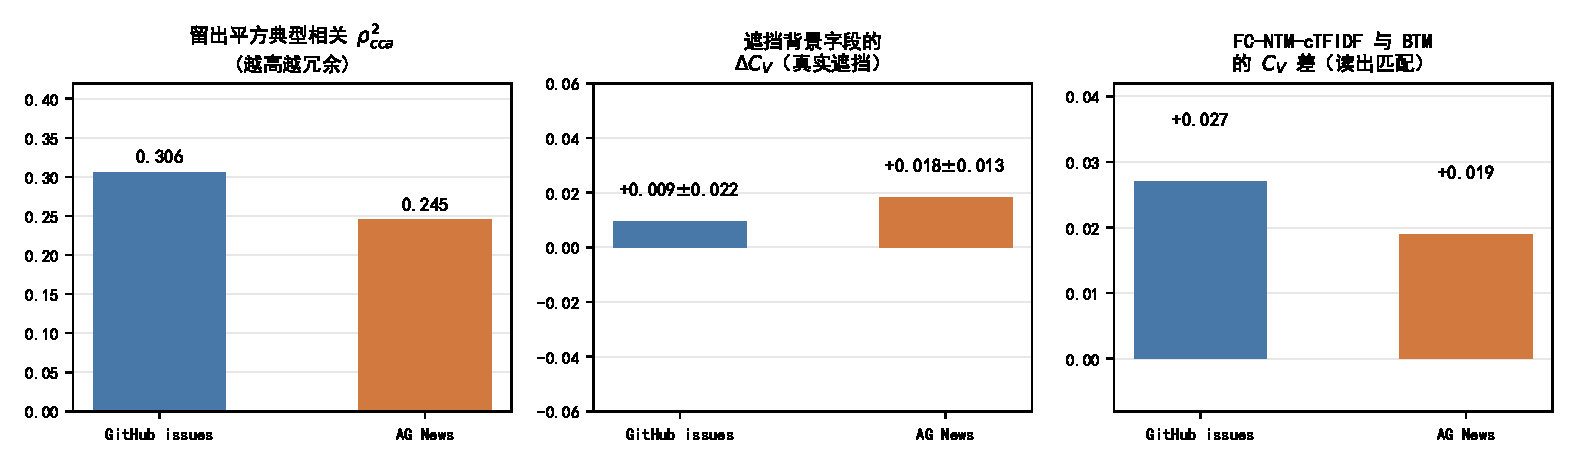
\includegraphics[width=0.86\textwidth]{fig_complementarity.pdf}
\caption{字段冗余度与增益的关系（留出度量）。左：留出平方典型相关
$\rho^2_{\mathrm{cca}}$（越高越冗余，训练集拟合、测试集评估）；中：\emph{真实}遮挡推断的
$\Delta C_V$（推理期把背景字段整体置零并重新推断，GitHub $+$0.009$\pm$0.022、
AG News $+$0.018$\pm$0.013，各 3 个种子）；
右：\fcntm{}-cTFIDF 与 BTM 的 $C_V$ 差（读出匹配口径，GitHub $+$0.027、
AG News $+$0.019）。
两个语料的冗余度接近，但 10 种子配对下增益只在 GitHub 上为正（AG News 为 $-$0.009），
因此该图不支持“冗余度预测增益”的结论。}
\label{fig:cond}
\end{figure}

\begin{table}[t]
\centering
\caption{GitHub issues 上 \fcntm{} 的主题样例（seed=11，$K=30$，best epoch 547，
表 \ref{tab:github} 与图 \ref{fig:main} 所用的同一模型）。词表内容由该主结果模型的
$\beta$ 与 $\theta$ 自动生成：先按式
\eqref{eq:ctfidf} 计算类 TF-IDF 读出，再分别截断到概要/背景字段词表，因此表中不含任何
词表外词；主题名由人工命名。}
\label{tab:topics}
\footnotesize
\setlength{\tabcolsep}{4pt}
\begin{tabular}{@{}p{2.7cm}p{5.9cm}p{5.9cm}@{}}
\toprule
主题（人工命名） & 概要侧核心词（前 10 个） & 背景侧核心词（前 10 个） \\
\midrule
% T03 (github, seed 11)
类型系统与语言服务 & type typescript function string types regression error property assignable array & type typescript function string types regression error property assignable array \\  % label=typescript mass=0.069
% T08 (github, seed 11)
DuckDB 构建与分发 & duckdb all python data sets distribution architecture linux required nightly & duckdb all python data reproducing sets distribution architecture linux required \\  % label=duckdb mass=0.055
% T05 (github, seed 11)
Redis 复制与集群 & master cluster redis node sentinel slave nodes docker failover command & master cluster redis node sentinel slave nodes docker failover command \\  % label=redis mass=0.035
% T07 (github, seed 11)
配置与命令语义 & redis command key set value some keys error one cluster & redis command key set value some keys error one cluster \\  % label=redis mass=0.050
% T09 (github, seed 11)
语言特性建议 & javascript type typescript suggestion types existing runtime change feature syntax & javascript type typescript suggestion types wouldn existing runtime change feature \\  % label=typescript mass=0.043
% T02 (github, seed 11)
事件循环与缓存指标 & idle addr sub flags cmd age multi free events name & qbuf psub oll obl idle addr sub flags cmd omem   % label=redis mass=0.007

\\   % the row terminator lives here, not in the \input file: a trailing \\
     % at the end of an \input-ed file breaks \bottomrule (Misplaced \noalign)
\bottomrule
\end{tabular}
\end{table}

\section{数据与指标说明}

\subsection*{数据说明}

三点需要一并说明。第一，预处理（去停用词与词表过滤）之后，训练划分与测试划分之间存在少量
\emph{完全相同的 token 序列}：GitHub 10 条、AG News 8 条（分别占测试集的 0.50\% 与 0.11\%）。
它们来自不同的原始记录，是过滤后退化重合，不是原始记录的重复（原始记录无重复）；这一比例
不足以改变本文结论，但读者应知悉该口径。第二，GitHub 的背景字段有很长的长尾：预处理后
训练集最长 8501、测试集最长 20532 个 token，而依赖句向量的基线会按预训练编码器的最大长度
截断，因此它们实际看到的信息少于词袋模型；本文除均值外在此同时报告该长尾。
第三，预处理后还有极少数记录\emph{概要字段变空}：GitHub 训练集 6 条、测试集 1 条，AG News
训练集 69 条、测试集 98 条（最高比例为测试集的 1.29\%）。这些记录仍保留在主表中，其概要侧
输入为空向量；需要说明的是，模型对\emph{概要}为空并没有像背景为空那样的显式回退分支——
概要编码器照常运行，其零输入会得到一个由训练参数决定的后验，再与背景后验门控融合
（用 seed 11 检查点实测：GitHub 那 1 条记录的融合后验与"只用背景后验"的最大差为 0.115、
最可能主题不变；AG News 的 98 条最大差 0.261、其中 3 条最可能主题改变）。因此本文的置零
训练与遮挡实验（第 \ref{sec:occlusion-robust} 节）验证的是\emph{背景}缺失下的行为，不能
直接外推到概要缺失；此处给出计数与实测差异，以便读者判断其影响范围。

\emph{注：}正文的长度、词表重叠、JS 与字段独有内容占比统一按正式划分（6000 条训练）
统计；开发阶段使用的 1000 条子样本对应统计量为 AG News 描述 13.1 / 标题 3.25，GitHub
正文 70.9 / 标题 5.24，该子样本上重建的词表规模为 1914 / 2682。

\textbf{开发子样本与最终评测集的重叠。}两个语料的设计迭代（门控与均值融合的取舍、融合
归一化方式、读出变体筛选）是在从\emph{正式测试划分}中抽出的 400 条小样本上完成的
（各语料 1000 训练 / 400 测试）。把包含这 400 条记录的完整测试
集当作完全未接触的确认集会产生选择偏差。本文的处理方式是把评测分成两套并同时报告：
(i) \emph{完整测试划分}，与基线结果使用同一划分；(ii)
\textbf{无开发重叠测试集}，即从完整测试划分中剔除上述 400 条后剩下的 1600 条（GitHub）
与 7200 条（AG News），由记录级精确匹配得到；一致性指标在每个已存模型的主题词表上
重新计算。后者是一份
\emph{重评分敏感性分析}：它只消除了\emph{直接}重叠，并不能撤销已经发生的模型与配置选择，
因此不构成“未接触过”的确认集；要得到独立确认，需要在方案冻结后用未参与开发的新仓库或新
语料评测，本文将其列为后续工作。

\subsection*{评价指标的补充定义}

其中 EXCL$_{\mathrm{KADJ}}$ 是本文对 Bischof--Airoldi 排他性的 K 校正变体：先按
\cite{bischof2012exclusivity} 的定义计算每个主题前 10 个词的列归一化质量均值
$\mathrm{EXCL}$，再映射为 $\mathrm{EXCL}_{\mathrm{KADJ}}=(\mathrm{EXCL}-1/K)/(1-1/K)$，
使其在随机主题下约为 0、完全排他时约为 1。该式是本文的定义而非原文的指标，正文与图中
均按此说明；它也并不消除不同 $K$ 之间以及不同分数矩阵之间的可比性问题，因此表中只对
固定 $K=30$ 的模型并列比较。
需要额外说明一处口径差异：对 \fcntm{}-cTFIDF 行，该列是在\emph{类 TF-IDF 得分矩阵}
（经行归一化后）上计算的，它不再是概率分布，因而与其它模型的 $\beta$ 行不是同一个量；
这张表与图只把它作为同一读出内部的排序参考，不对 cTFIDF 行与 $\beta$ 行之间的大小关系
作解释。

IRBO 采用有限长度外推形式：截断项之外补上残差尾项，
\begin{equation}
\mathrm{RBO}_{\mathrm{ext}}=(1-p)\sum_{d=1}^{L}p^{d-1}A_d
+p^{L}A_L ,
\label{eq:rbo}
\end{equation}
其中 $p=0.9$、$L$ 为共同深度、$A_d$ 为前 $d$ 位的集合重叠率，主题多样性取
$\mathrm{IRBO}=1-\overline{\mathrm{RBO}}_{\mathrm{ext}}$。不加尾项时两张完全相同的 10 词
主题表也会得到 $1-p^{L}=0.651$ 的“相似度”（多样性 0.349）；按最终深度的重叠程度不同，
该偏置对不同主题对的幅度不同（完全重叠时为 $p^{L}$，完全不相交时为 0），因此它不是给所有
模型叠加的同一常数。

\end{document}
